%-----------------------------------------------------------------------------%
\chapter{ANALISIS DAN PERANCANGAN SISTEM}
%-----------------------------------------------------------------------------%
\vspace{4.5pt}

Pada bab ini menjelaskan analisis masalah yang diatasi, alur kerja dari perangkat lunak yang dikembangkan, arsitektur dan metode yang digunakan serta hasil evaluasi

\section{Analisis Masalah}
Arsitektur ERP yang digunakan pada Odoo yaitu arsitektur Service Oriented Architecture (SOA) dan masih dideploy secara monolit, seperti yang sudah dijelaskan pada landasan teori. Arsitektur monolit memiliki kelemahan dan permasalahan yang bisa diselesaikan dengan arsitektur microservice. Aplikasi ERP juga diperlukan untuk memiliki skalabilitas yang baik dan kustomisasi.

Namun untuk melakukan perubahan arsitektur harus dilakukan dekomposisi, proses dekomposisi sendiri tidak mudah karena proses dekomposisi masih membutuhkan analisis secara manual dan untuk mengidentifikasi service sulit karena banyaknya pendekatan dan pertimbangan.
Pada penelitian ini menggunakan pendekatan Hierarchical clustering untuk membantu menemukan service yang tepat, dimana hierarchical clustering memberikan rekomendasi bagaimana pengelompokan service berdasarkan pemilihan partisi terbaik.
Proses dimulai dari melalukan analisis kode seperti Call Graph yang dihasilkan dari kode aplikasi Odoo. Hasil analisis kode di ekstraksi menjadi matrix untuk dilakukan hierarchical clustering. Cluster terbaik dipilih melalui nilai secara struktural yaitu nilai coupling  dan kohesi.

Hasil terbaik dari clustering diimplementasikan menjadi service, penelitian ini akan menggunakan strategi dengan pola strangle untuk memecah kode di monolit. Untuk dekomposisi pada data akan menggunakan strategi Aggregate Exposing Monolith. Agar data antar service tetap terintegrasi maka dilakukan penerapan SAGA dengan pendekatan Orchestrated .

Microservice yang dibentuk akan dievaluasi melalui uji beban dan penggunaan sumber daya aplikasi untuk menentukan apakah dengan arsitektur microservice dapat menyelesaikan permasalahan yang muncul pada arsitektur monolit di aplikasi ERP.
\\

\section{Kerangka Pemikiran}
\begin{center}
	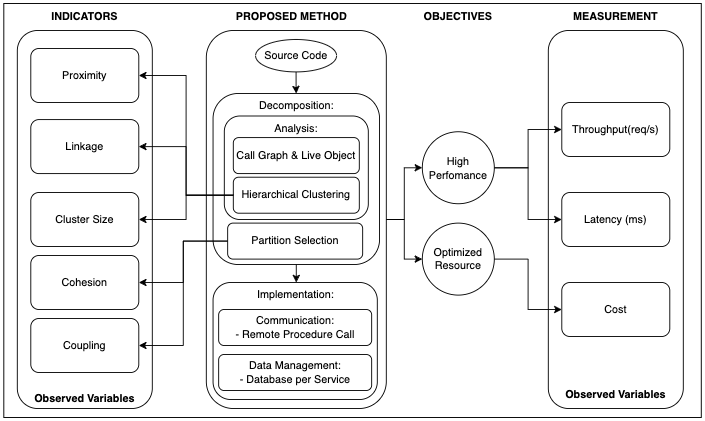
\includegraphics[width=14cm]{img/KerangkaPemikiran.png}
	\captionof{figure}{Kerangka Pemikiran}
	\label{fig:asd}
\end{center}

Penelitian akan dimulai dengan menggunakan kode sumber aplikasi yang dibuat dengan monolit. Kode sumber dilakukan proses dekomposisi yaitu dengan analisis seperti mencari objek beserta atributnya, untuk mencari keterhubungan lebih lanjut tentang objek maka dilakukan pencarian pada fungsi-fungsi sehingga terbentuklah graph yang menunjukan bagaimana keterhubungan masing-masing objek di aplikasi.

Dari graph yang sudah dibuat akan dilakukan pengelompokan dengan pendekatan Hierarchical Clustering. Dimana perlu ditentukan cara menghitung kedekatan antara objek dan pemilihan algoritma Linkage. Metode linkage yaitu menentukan jarak atau kemiripan antara semua objek. Untuk menentukan jarak ini bisa dengan rata-rata, maximum, minimum dan mengecilkan variance.

Pengelompokan dari Hierarchical Clustering akan dipilih dengan mencari nilai cohesion terendah dan  nilai coupling tertinggi. Dimana Internal Coupling mengevaluasi tingkat ketergantungan langsung dan tidak langsung antar objek. Semakin banyak dua objek menggunakan metode masing-masing semakin mereka menjadi satu kesatuan. Sedangkan Internal Cohesion akan mengevaluasi kekuatan interaksi antar objek. Biasanya, dua objek atau lebih menjadi interaktif jika metodenya bekerja pada atribut yang sama.

Ketika analisis dekomposisi sudah selesai dilakukan maka akan dilakukan implementasi berdasarkan pengelompokannya masing-masing yang akan menjadi service. Untuk metode komunikasinya antara service yaitu dengan Remote Procedure Call(RPC) dan untuk mengelola data, setiap service memiliki databasenya masing-masing dan untuk menjaga konsistensi data antar service maka digunakan pendekatan SAGA dengan cara choreography.

Untuk mengetahui bagaimana performa dari microservice dibandingkan dengan monolit yaitu dengan test beban. Pengukuran performa dilihat dari throughput, jumlah response, dan latency. 


\section{Urutan Proses Global}
\begin{center}
	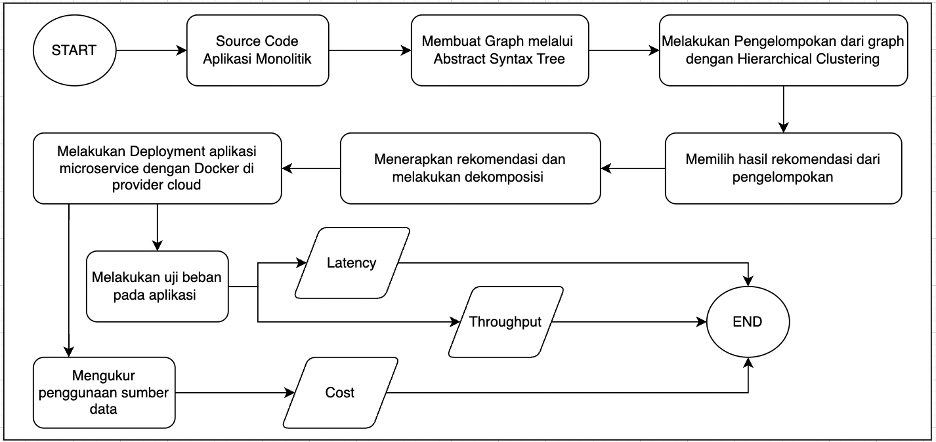
\includegraphics[width=14cm]{img/FlowchartProsesGlobal.png}
	\captionof{figure}{Diagram Flowchart Proses Global }
	\label{fig:asd}
\end{center}

\subsection{Proses Clustering}

\subsubsection{Pengambilan Source Code}
Aplikasi ERP Odoo merupakan aplikasi berlisensi open source, kode program dapat diunduh melalui situs repository Odoo. Pada tugas akhir ini menggunakan Odoo versi 16 dengan status pengujian lulus. Agar kode program dapat berjalan dengan lancar maka diperlukan proses installasi library, module dan Package yang digunakan dari file requirement.txt
\begin{center}
	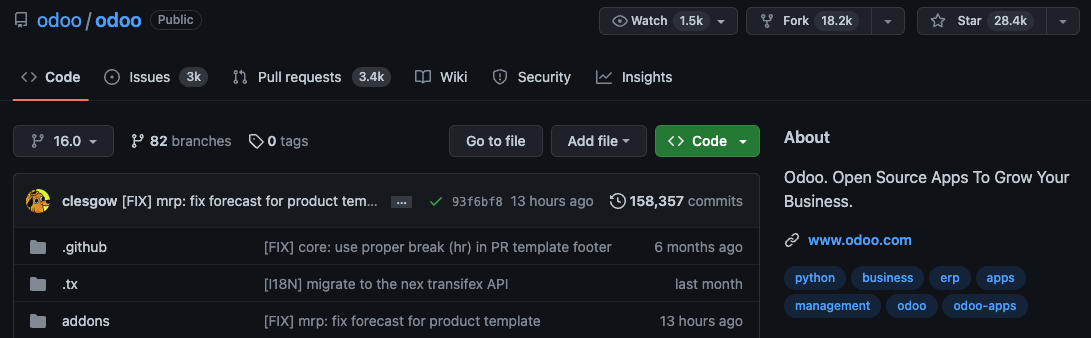
\includegraphics[width=14cm]{img/bab_3/github.png}
	\captionof{figure}{Source Code Aplikasi Odoo pada git repository}
	\label{fig:asd}
\end{center}
\subsubsection{Pembuatan Call Graph}
Pada tugas akhir ini menggunakan tools PyCG untuk menghasilkan call graph dalam bentuk format JSON. Adapun beberapa modifikasi perlu dilakukan pada tools PyCG yaitu pada module classes di class ClassNode dengan tujuan mencegah terjadinya pengulangan tak terbatas pada kasus \textit{Monkey Patching}.
\begin{center}
	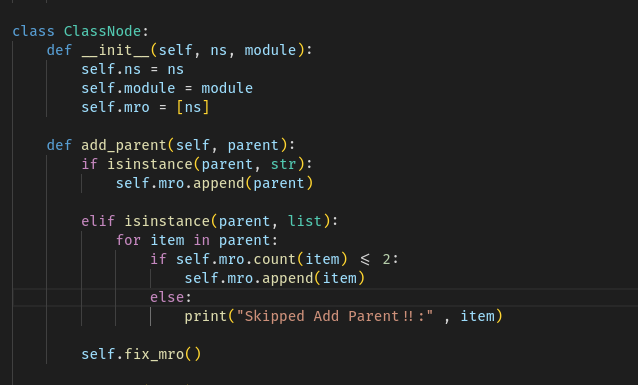
\includegraphics[width=14cm]{img/bab_3/ModifiedPyCG.png}
	\captionof{figure}{Class yang dimodifikasi pada PyCG}
	\label{fig:asd}
\end{center}
\begin{center}
	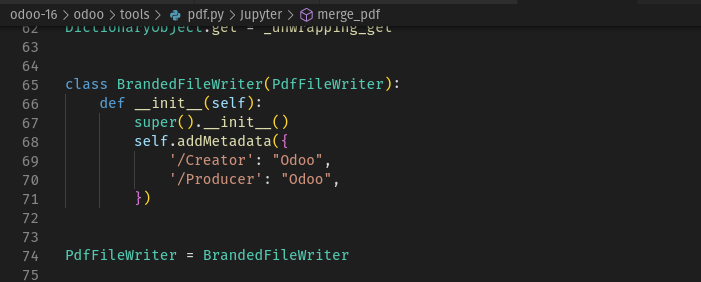
\includegraphics[width=14cm]{img/bab_3/MonkeyPatch.png}
	\captionof{figure}{Kasus Monkey Patching di Odoo}
	\label{fig:asd}
\end{center}
Terdapat 2 target folder yang dibuat call graph yaitu folder odoo dan folder addons karena folder lainnya tidak memiliki hubungan mengenai proses bisnis. Untuk menghemat waktu pembuatan call graph pada folder test tidak diikutkan.  Entry point untuk tools PyCG adalah semua file di target folder dengan extensi file .py serta ditentukan package yang ingin diolah menjadi call graph. Proses eksekusi dilakukan melalui terminal. Call graph yang dihasilkan berisi call yang berasal dari file .py yang ditentukan sebelumnya dan semua module yang terhubungan dari target. Semua module ini bisa diluar dari target module apabila keterhubungan itu terus berlanjut. PyCG hanya bisa menghasilkan call graph tanpa informasi mengenai jumlah pemanggilan dan urutan pemanggilan.
\begin{center}
	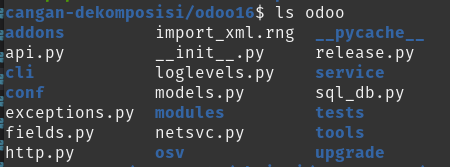
\includegraphics[width=9cm]{img/bab_3/lsOdoo.png}
	\captionof{figure}{Isi folder Odoo}
	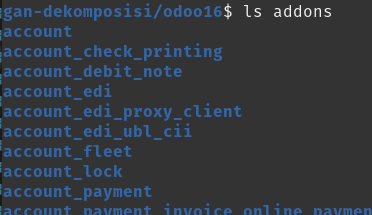
\includegraphics[width=9cm]{img/bab_3/lsAddons.png}
	\captionof{figure}{Isi folder Addons}
	\label{fig:asd}
\end{center}

\subsubsection{Ekstraksi Call Graph}
Proses ekstraksi json yang dihasilkan dari tools PyCG berupa 2 file JSON masing masing adalah odoo dan addons. Kedua file JSON digabungkan dan menjadi satu graph yang direpresentasikan dalam bentuk adjacency list di python.
\begin{center}
	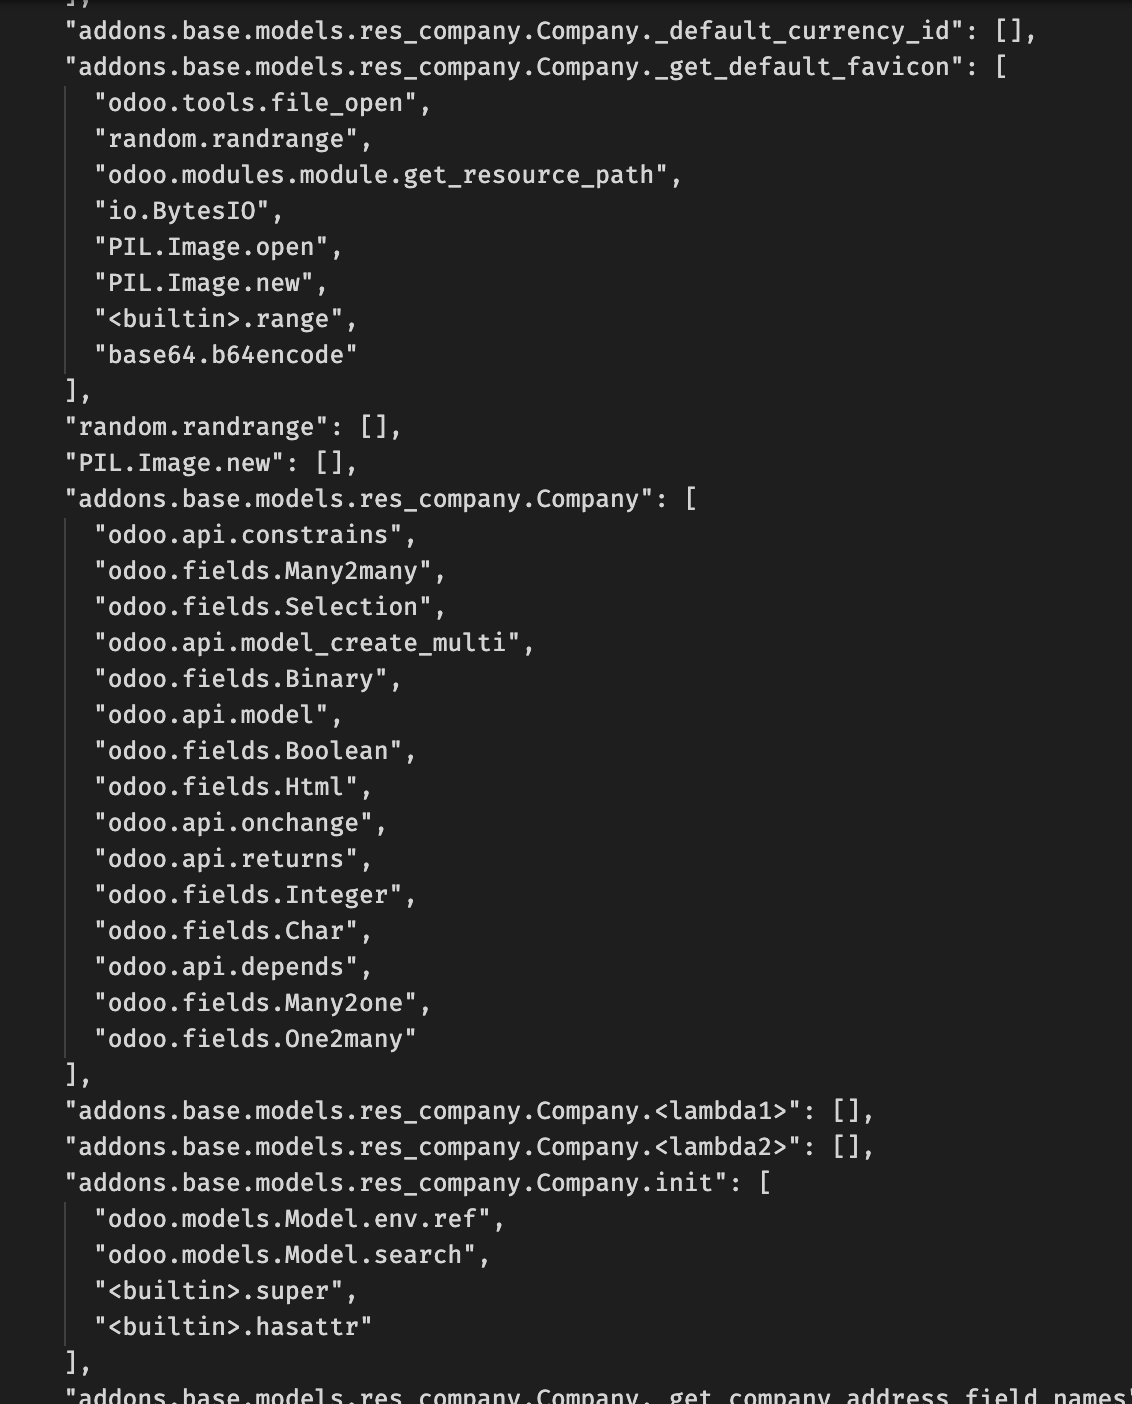
\includegraphics[width=9cm]{img/bab_3/JSONPyCG.png}
	\captionof{figure}{Ilustrasi JSON yang dihasilkan PyCG}
	\label{fig:asd}
\end{center}
\subsubsection{Ekstraksi Depedency Module}
Keterbatasannya informasi call graph yang dihasilkan dari PyCG, sehingga tugas akhir ini  menggunakan library python yaitu 'inspect' untuk menganalisis object secara run-time. Hal ini disebabkan python adalah bahasa pemrogram dynamic dimana pengecekan tipe data dilakukan secara 'run-time'. Ektrasi ini difokuskan pada module yang memiliki proses bisnis baik seperti module addons dan odoo/addons.
\begin{center}
	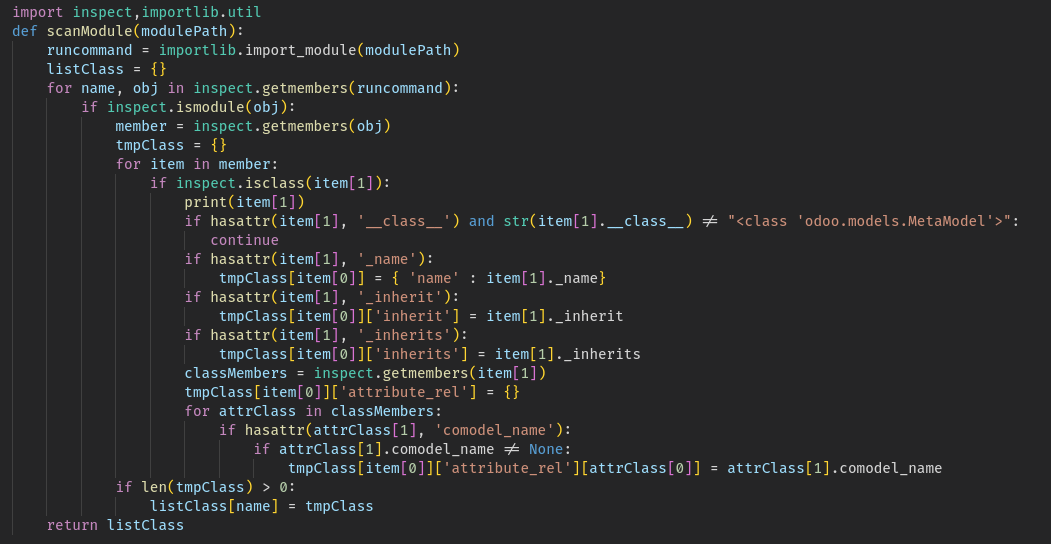
\includegraphics[width=14cm]{img/bab_3/InspectScan.png}
	\captionof{figure}{Implementasi inspect untuk mengekstraksi object di addons Odoo}
	\label{fig:asd}
\end{center}
Object yang dianalisis yaitu class yang merupakan turunan dari class odoo.models.MetaModel, dimana class MetaModel memiliki properties seperti  name, \_inherits , \_inherit, dan attribute\_rel. Hasil ekstrasi depedency module digabungkan melalui nama module PyCG 
\\
\subsubsection{Pre Procesinng}
Graph yang dihasilkan dari proses ekstrasi dipisahkan antara module eksternal dan module internal. Module yang digunakan untuk pengelompokan adalah module internal, setiap call yang dilakukan memiliki nama call yang berupa gabungan antara nama fungsi / class / module /file di kode program. PyCG tidak memberikan informasi apakah nama call tersebut berupa tipe apa, untuk itu pengelompokan dilakukan secara Hybrid yaitu berdasarkan module dan file. 

Nama call yang disatukan menjadi module adalah call yang memiliki awalan(root) addons atau odoo/addons dan nama call yang disatukan dengan file adalah nama call selain addons. Call yang dikelompokan memiliki nilai agregasi dari jumlah call. Jumlah call dapat digunakan sebagai weight yang dapat menunjukan kekuatan antara call satu sama lain, proses ini membentuk call baru yang lebih ringkas dan relevan dalam bentuk graph. Proses visualisasi call graph dilakukan melalui tools graphViz.
\begin{center}
	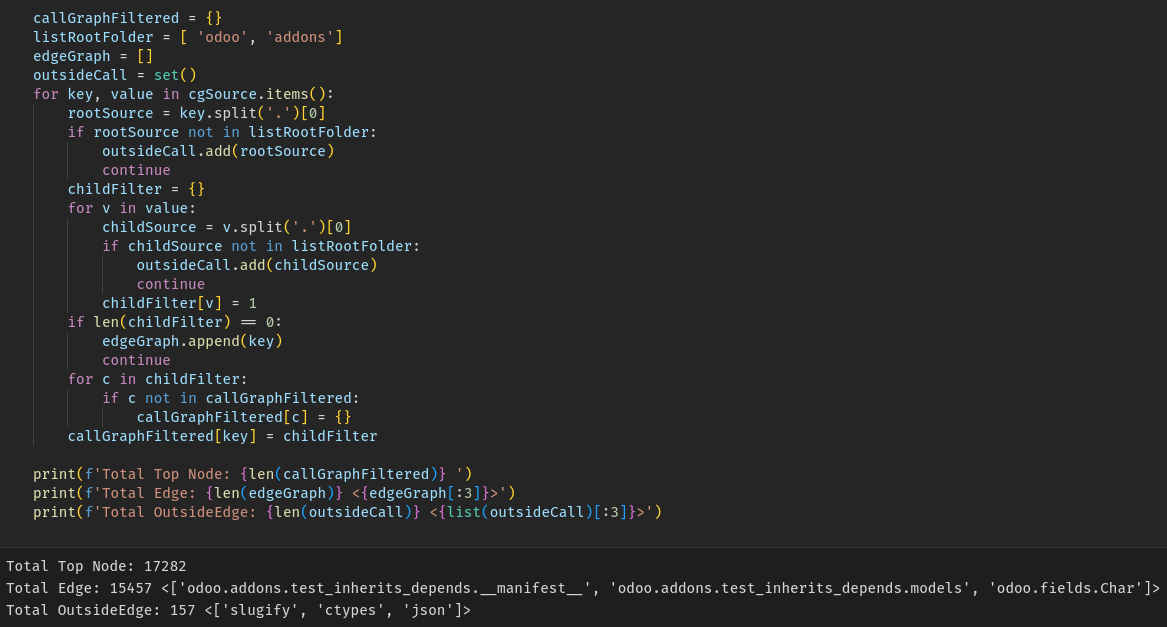
\includegraphics[width=14cm]{img/bab_3/filterCG.png}
	\captionof{figure}{Menghilangkan Node diluar dari target}
	\label{fig:asd}
\end{center}

\subsubsection{Hierarchical Clustering}
Graph yang berbentuk Adjacency list diubah menjadi adjacency matrix, proses normalisasi data dilakukan pada matrix. Yang kemudian matrix tersebut dibuat menjadi Distance Matrix, rumus jarak yang digunakan ada 3 yaitu Jaccard, Hamming dan Struktural. Masing-masing hasil jarak disatukan dengan rata-rata. 
\begin{center}
	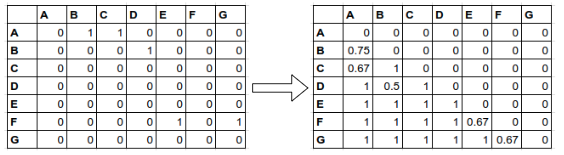
\includegraphics[width=9cm]{img/bab_3/simJaccard.png}
	\captionof{figure}{Jarak Jaccard}
	\label{fig:asd}
\end{center}
\begin{center}
	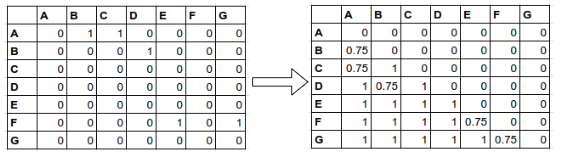
\includegraphics[width=9cm]{img/bab_3/simStr.png}
	\captionof{figure}{Jarak Struktural}
	\label{fig:asd}
\end{center}
\begin{center}
	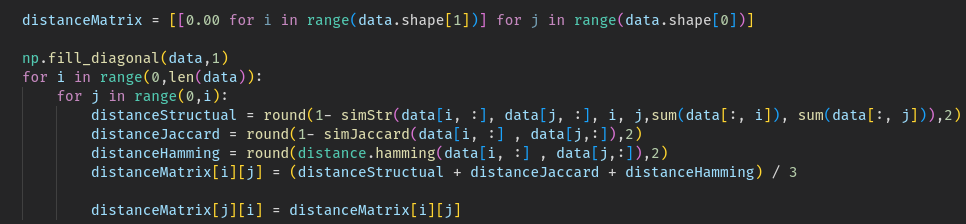
\includegraphics[width=14cm]{img/bab_3/distanceMatrix.png}
	\captionof{figure}{Pembuatan Distance Matrix}
	\label{fig:asd}
\end{center}

Distance Matrix dapat dilihat nilai dengan ilustrasi Heatmap, dimana sumbu x dan y adalah semua module dan nilai kedekatanya dengan module lainnya. Pada tugas akhir ini menggunakan library SciPy yang memiliki fungsi Hierarchical Clustering dengan algoritma linkage. Hasil pengelompokan dapat ditampilan dalam bentuk dendogram.
\begin{center}
	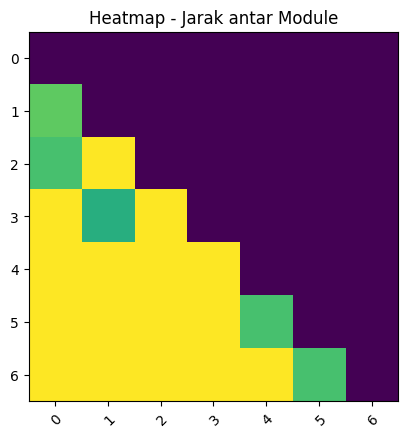
\includegraphics[width=10cm]{img/bab_3/heatmap.png}
	\captionof{figure}{Ilustrasi Heatmap}
	\label{fig:asd}
\end{center}
\begin{center}
	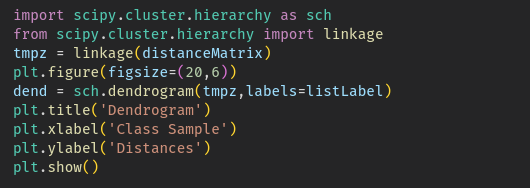
\includegraphics[width=14cm]{img/bab_3/Clustering.png}
	\captionof{figure}{Proses Pengelompokan}
	\label{fig:asd}
\end{center}

\subsubsection{Pemilihan Partisi}
Pemilihan jumlah cluster/partisi perlu dilakukan dengan perhitungan yang dapat menentukan jumlah service yang ideal. Microservice yang ideal memiliki nilai coupling yang rendah dan nilai kohesi yang tinggi. Untuk itu tugas akhir ini menentukan partisi secara nilai struktural. 
\begin{center}
	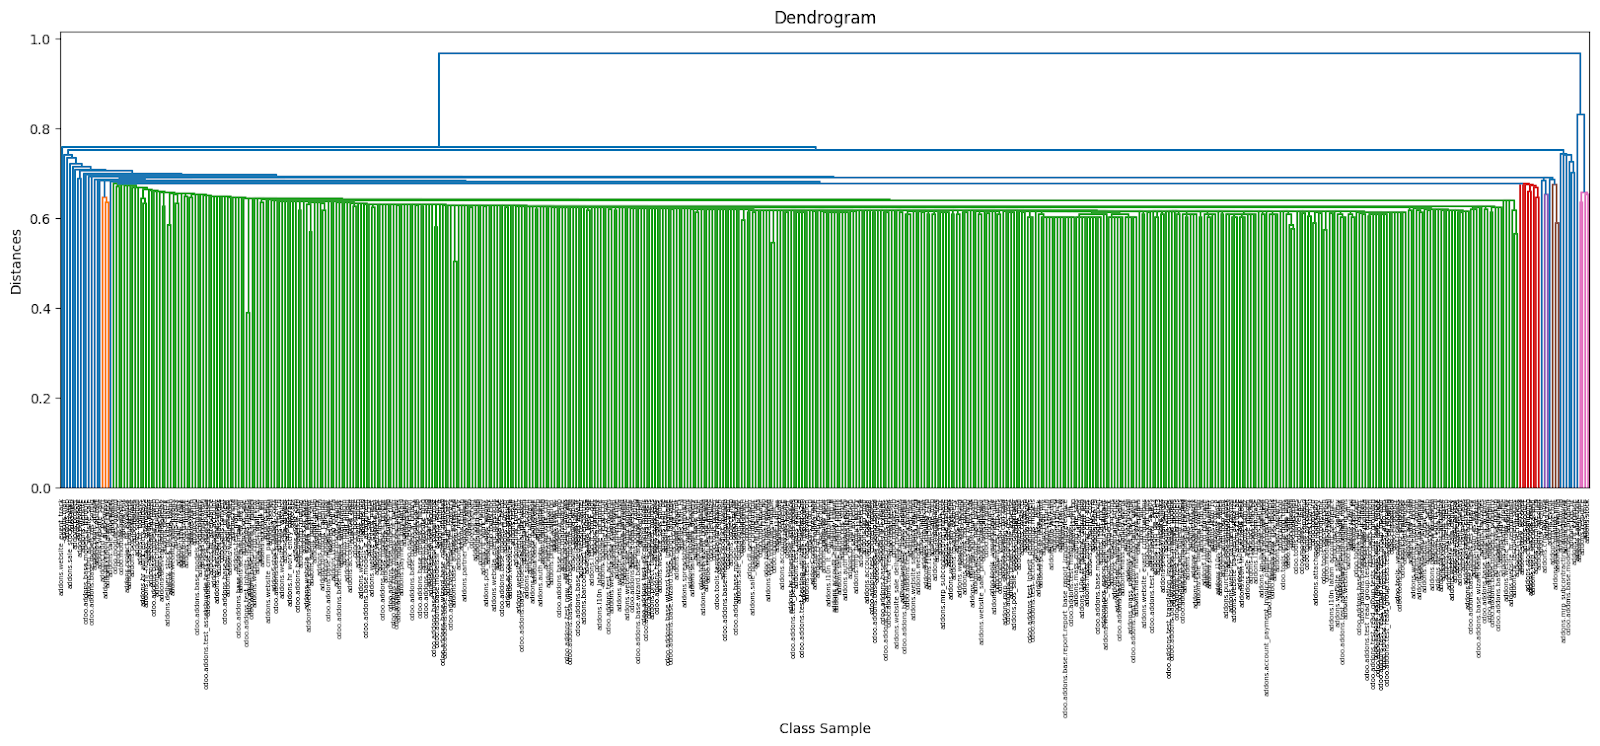
\includegraphics[width=14cm]{img/bab_3/dendogram.png}
	\captionof{figure}{Dendogram yang dihasilkan dari Clustering}
	\label{fig:asd}
\end{center}
Terdapat implementasi rumus yang digunakan FOne, InterCoup, Inter Coh dan NBCalls. Nilai FOne  yang menentukan apakah partisi dengan jumlah cluster tertentu miliki nilai coupling dan cohesion yang ideal. Terdapat modifikasi rumus pada FOne yaitu adanya pembagian jumlah cluster pada nilai cohesion agar microservice yang memiliki banyak service lebih baik dari pada service yang sedikit sehingga  microservice yang dibentuk bisa independen. 
\begin{center}
	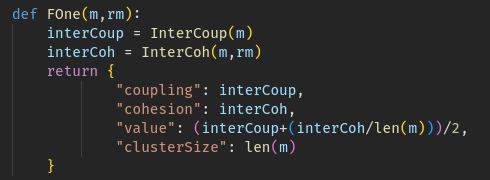
\includegraphics[width=14cm]{img/bab_3/FOne.png}
	\captionof{figure}{Implementasi FOne}
	\label{fig:asd}
\end{center}

Pada InterCoup yaitu menghitung coupling antara partisi. Perhitungan call antar partisi dihasilkan dari nama call, nama call sebelumnya yang mungkin mengarah ke nama call dimana nama call tersebut sudah menjadi bagian besar dari partisi lain. Maka nama call tersebut diganti menjadi nama call partisi itu, jumlah call yang terjadi tetap disimpan dan dibuat adjacency matrix baru untuk menghitung call dengan bantuan fungsi CoupP.
\begin{center}
	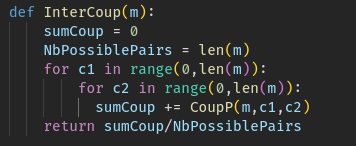
\includegraphics[width=14cm]{img/bab_3/InterCoup.png}
	\captionof{figure}{Implementasi InterCoup}
	\label{fig:asd}
\end{center}
Fungsi CoupP menghitung berapa nilai coupling antara kedua class dengan class lainnya. Coup menggunakan fungsi NBCalls untuk mengetahui berapa jumlah relasi antara kedua class tersebut.
\begin{center}
	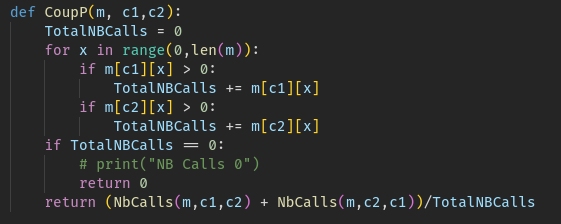
\includegraphics[width=14cm]{img/bab_3/CoupP.png}
	\captionof{figure}{Implementasi Coup}
	\label{fig:asd}
\end{center}

InterCoh menghitung cohesi dari setiap partisi di microservice. Setiap partisi yang dibentuk bila memiliki call maka call tersebut dihitung sebagai koneksi langsung dan koneksi tidak langsung ketika call diluar dari partisinya sendiri.
\begin{center}
	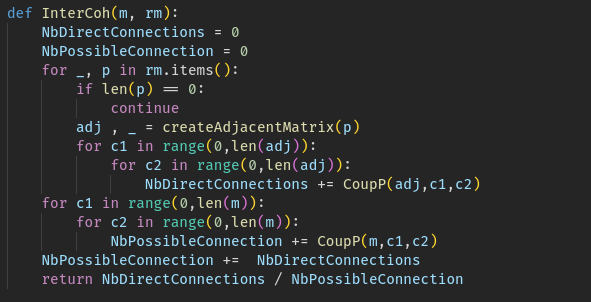
\includegraphics[width=14cm]{img/bab_3/InterCoh.png}
	\captionof{figure}{Implementasi InterCoh}
	\label{fig:asd}
\end{center}

Proses pencarian jumlah cluster dilakukan dari 1 cluster hingga semua cluster hanya memiliki 1 objek. dimulai dari pemotongan \textit{tree} dan menggabungkan class yang bersatu pada partisinya masing-masing dan kemudian memangil fungsi Fone. FOne menghasilkan nilai terendah (mendekati 0) adalah jumlah cluster yang terbaik untuk microservice.

\begin{center}
	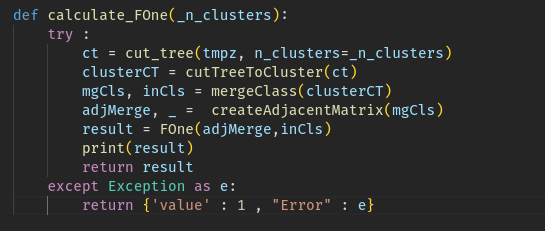
\includegraphics[width=14cm]{img/bab_3/FOneMultiCore.png}
	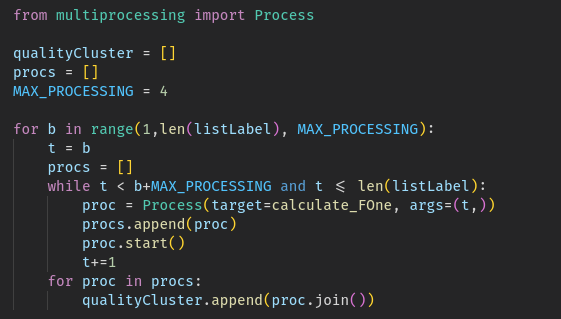
\includegraphics[width=14cm]{img/bab_3/BruteForceSearch.png}
	\captionof{figure}{Penerapan Pemilihan Jumlah Cluster terbaik}
	\label{fig:asd}
\end{center}

Berikut adalah nilai coupling dan cohes masing-masing jumlah cluster. Semakin tinggi jumlah cluster maka nilai coupling akan meningkat dan begitupula sebaliknya untuk nilai cohesion. Dari hasil yang ditemukan bahwa cluster yang ideal berjumlah 8-15 service.

\begin{center}
	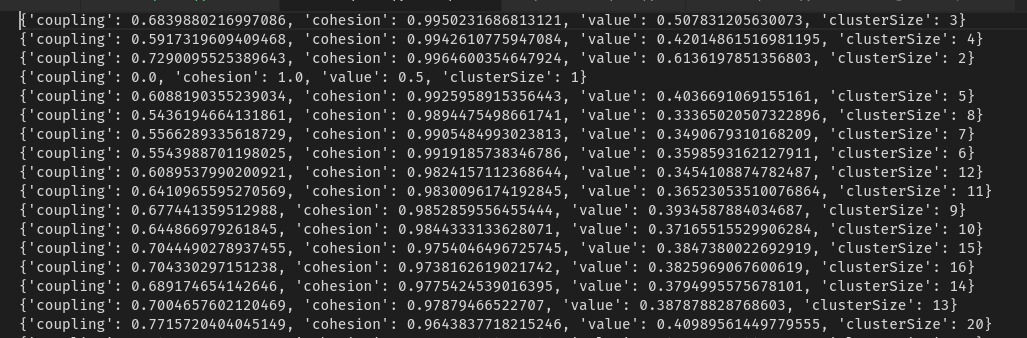
\includegraphics[width=14cm]{img/bab_3/ResGood.png}
	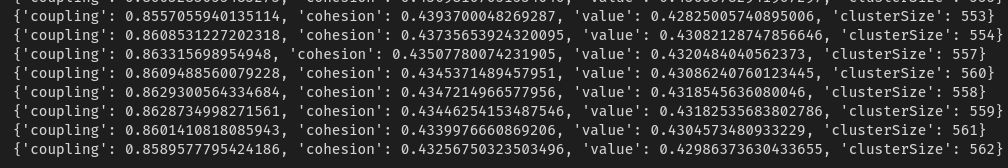
\includegraphics[width=14cm]{img/bab_3/ResBad.png}
	\captionof{figure}{Nilai Coupling dan Cohesion setiap jumlah cluster}
	\label{fig:asd}
\end{center}

\subsection{Dekomposisi Monolitik ke Microservice}
\subsubsection{Pemisahan User Interface}
Odoo adalah aplikasi ERP berbasis web, tampilan pada Odoo bisa dibuka pada broser yang kompatibel. Odoo menggunakan pendekatan SPA (Single Page Application) dan adanya server rendering untuk menghasilkan HTML. UI dapat memanggil API yang berada pada server yang sama, sehingga diperlukan pemisahan kepentingan. Benefit dari proses ini dapat meningkatan skalabilitas dan pengembangan bisa dilakukan secara independen.
\begin{center}
	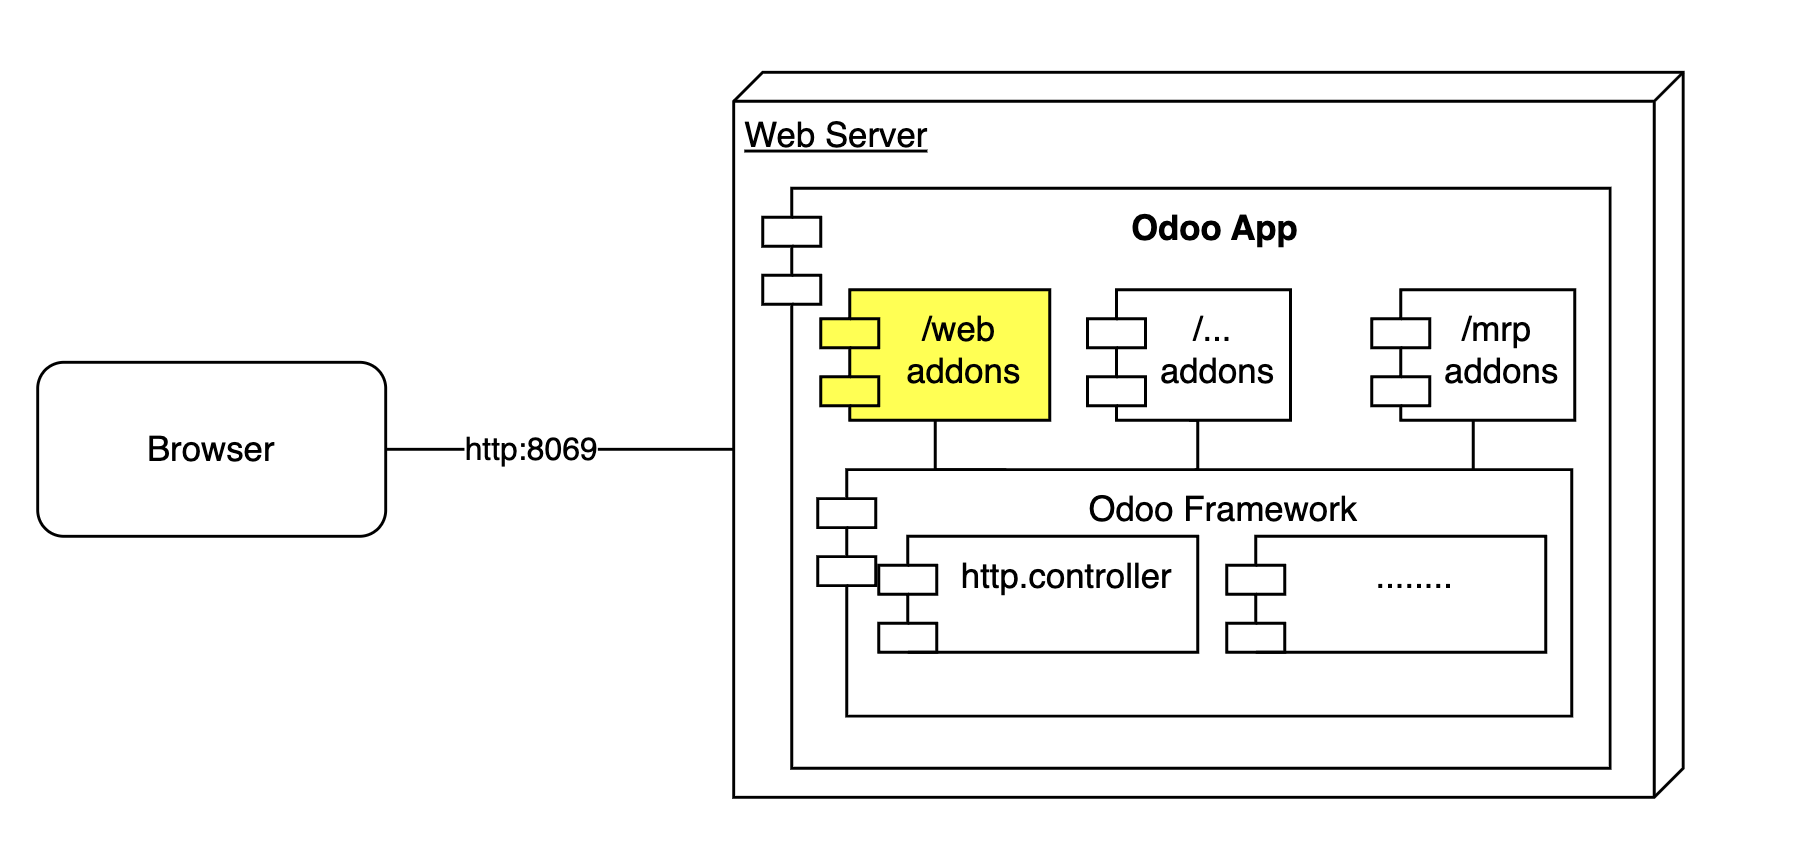
\includegraphics[width=14cm]{img/bab_3/monoUI.png}
	\captionof{figure}{Arsitektur UI Monolit}
	\label{fig:asd}
\end{center}
Proses pemisahan membutuhkan reverse proxy yang dapat menghubungkan web server dimana bertanggung jawab pada hal seperti file static(css,js,gambar) dan UI dengan web server lainnya. Tujuan adanya reverse proxy agar client hanya perlu mengetahui satu pintu masuk aplikasi yaitu reverse proxy itu sendiri dan tidak perlu mengetahui seluruh server yang ada di aplikasi.
\begin{center}
	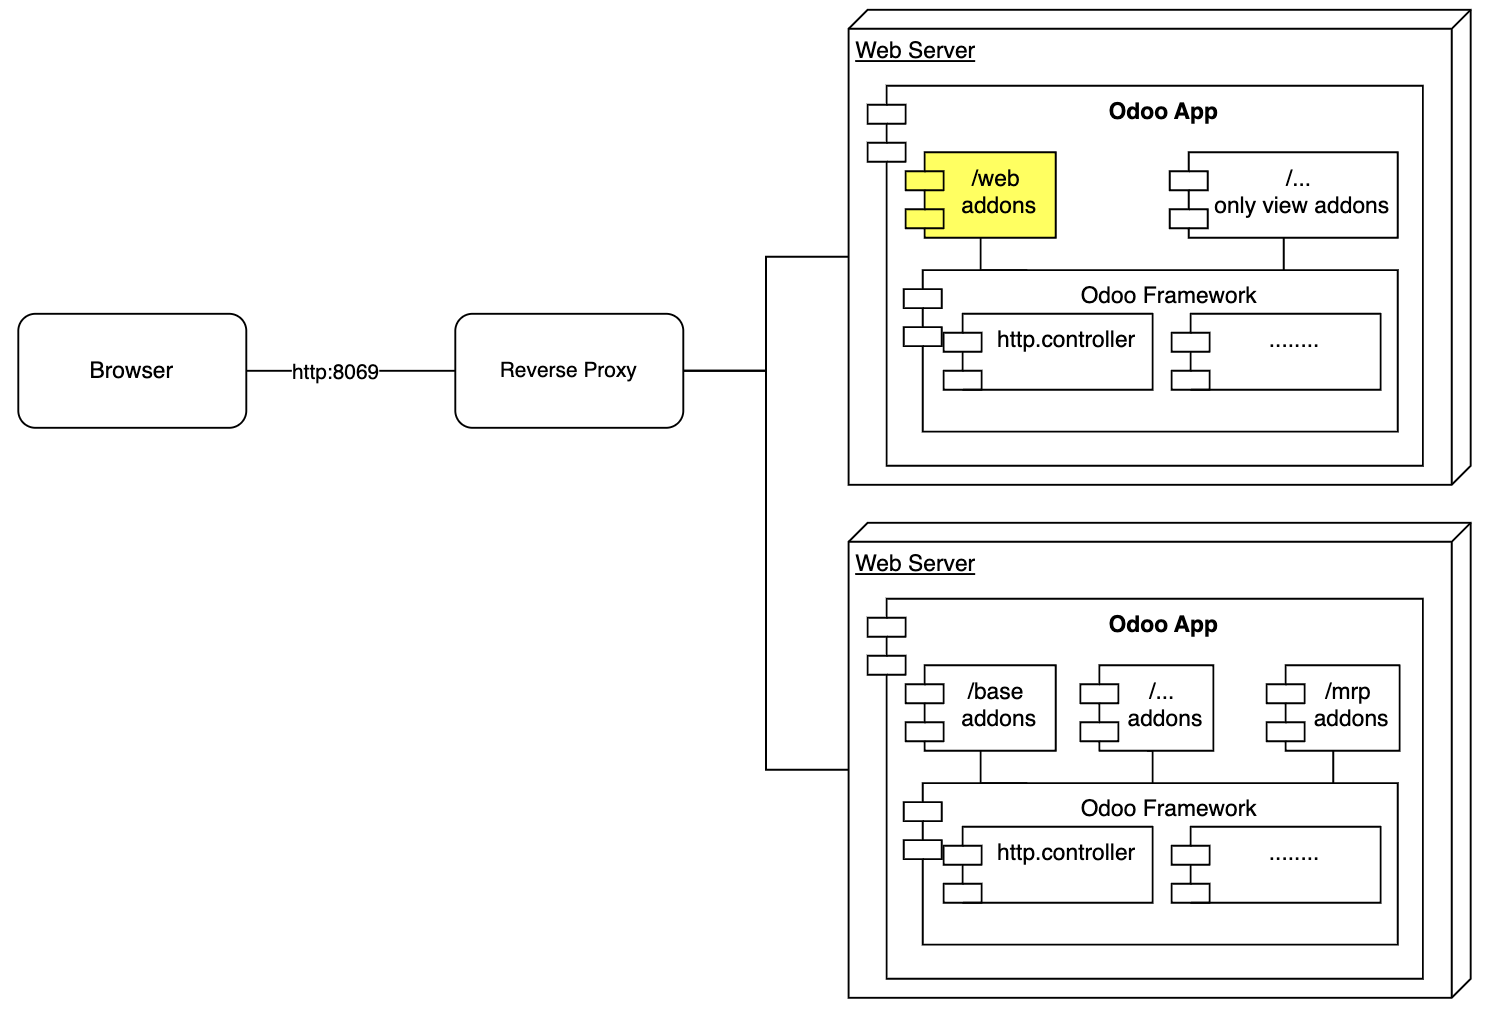
\includegraphics[width=14cm]{img/bab_3/microUI.png}
	\captionof{figure}{Arsitektur UI di Microservice}
	\label{fig:asd}
\end{center}

\subsubsection{Strategi Pemisahan Kode}
Berdasarkan landasan teori terdapat beberapa strategi pemisahan kode aplikasi monolit, pada tugas akhir ini akan menggunakan 2 strategi yaitu pola Strangle dan pola Branch by Abstraction. Pola Strangle diterapkan karena pendekatan ini umum diterapkan dan lebih mudah pada suatu aplikasi yang sudah besar, dengan pola ini aplikasi monolit bisa berdiri bersamaan dengan service yang ingin dibangun atau dimigrasi. 
\begin{center}
	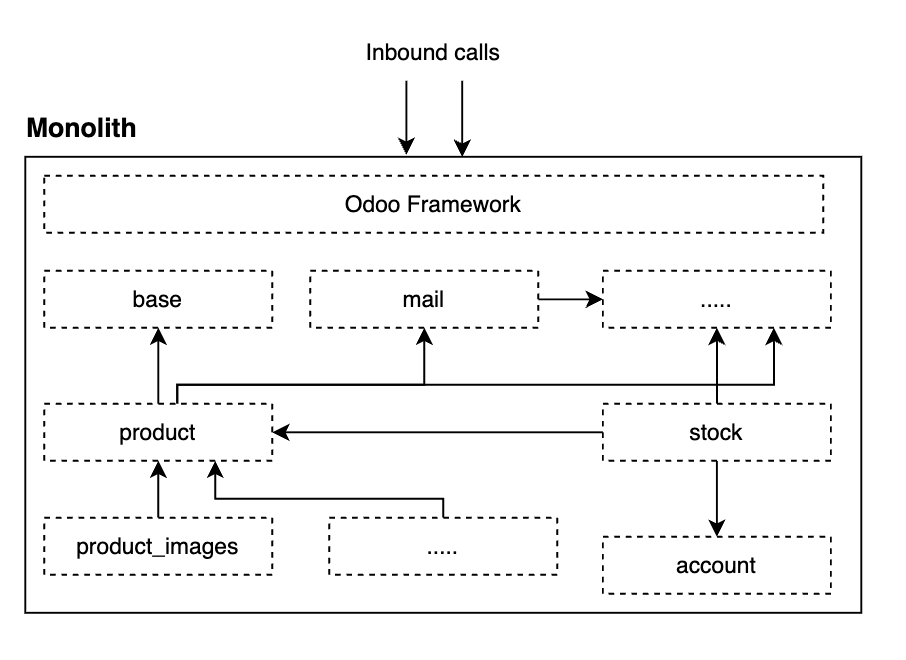
\includegraphics[width=14cm]{img/bab_3/strangelExMono.png}
	\captionof{figure}{Struktur Module dan Keterhubungannya di Aplikasi Monolit}
	\label{fig:asd}
\end{center}

Terdapat 3 langkah utama dalam menerapkan pola strangle yaitu memilih bagian yang ingin dipindahkan, memindahkan aplikasi menjadi service yang berdiri sendiri, dan yang terakhir mengubah call dari monolith ke service yang baru dibuat. Tugas akhir ini milih bagian yang dipindahkan pada kasus bisnis yaitu 'Product', Product bisa dilakukan penambahan Product baru, perubahan atributnya, pencarian atau mendapatkan product dan penghapusan product.

Proses pemindahan module dibantu dengan hasil clustering yang sudah diproses sebelumnya sehingga dibuat untuk membuat microservice. Untuk menghubungkan antara bagian yang sudah dipisah dari monolit dengan bagian yang masih di monolit maka diperlukan penerapan pola Branch by Abstraction. Terdapat dua bagian utama yaitu abstract dan adapter. Abstract berperan menggantikan bagian yang sudah pisah menjadi service sehingga bagian lain di monolit tidak terdampak dan Adapter adalah implementasi sesungguhnya yang menghubungkan antara service dan aplikasi monolith.
\begin{center}
	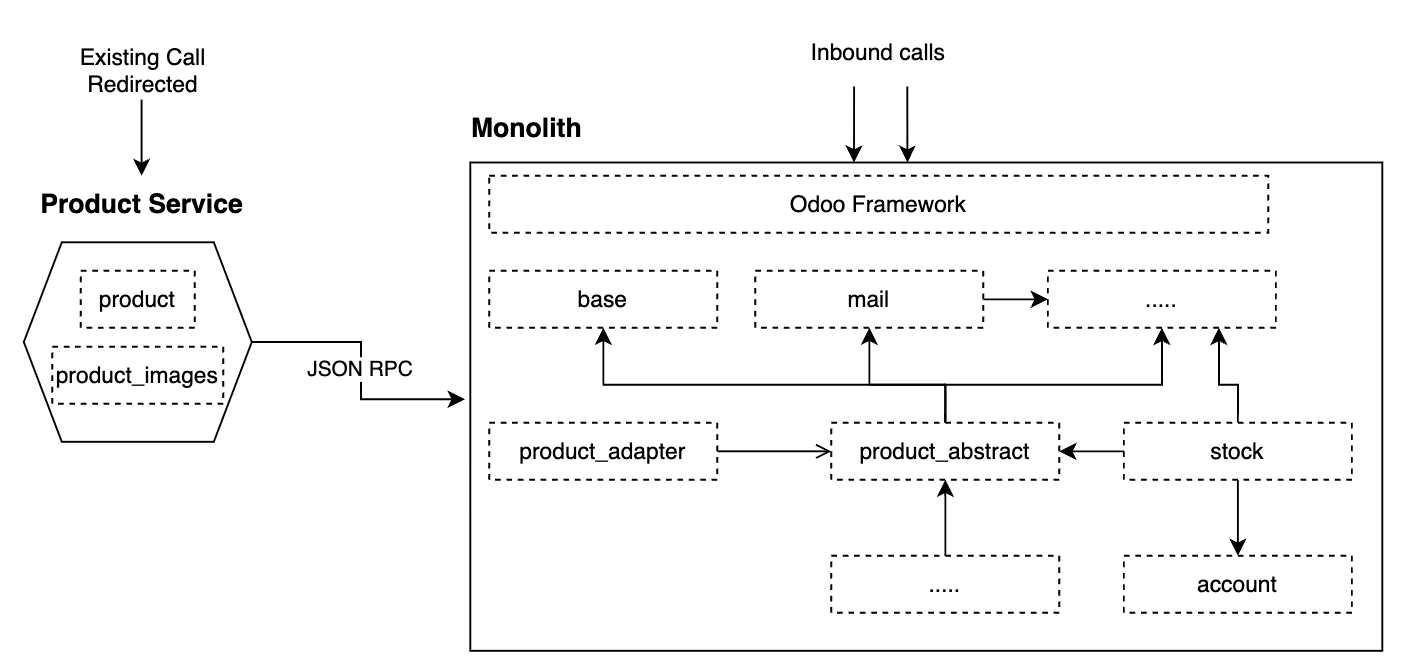
\includegraphics[width=14cm]{img/bab_3/strangelExMicro.png}
	\captionof{figure}{Penerapan Pola Strangle dan Branch by Abstraction}
	\label{fig:asd}
\end{center}
Pemisahan kode mempengaruhi proses autentikasi, proses autentikasi pada aplikasi Odoo terdapat 2 cara yaitu melalui password atau API-Key. Odoo menyimpan sesi autentikasi di cookie namun bukan dalam format JWT tapi bentuk HTTP session. Untuk itu diperlukan modifikasi pada sistem autentikasi yang menggunakan format JWT agar setiap service tidak perlu menvalidasi berkali-kali apakah sesi itu valid. 
\begin{center}
	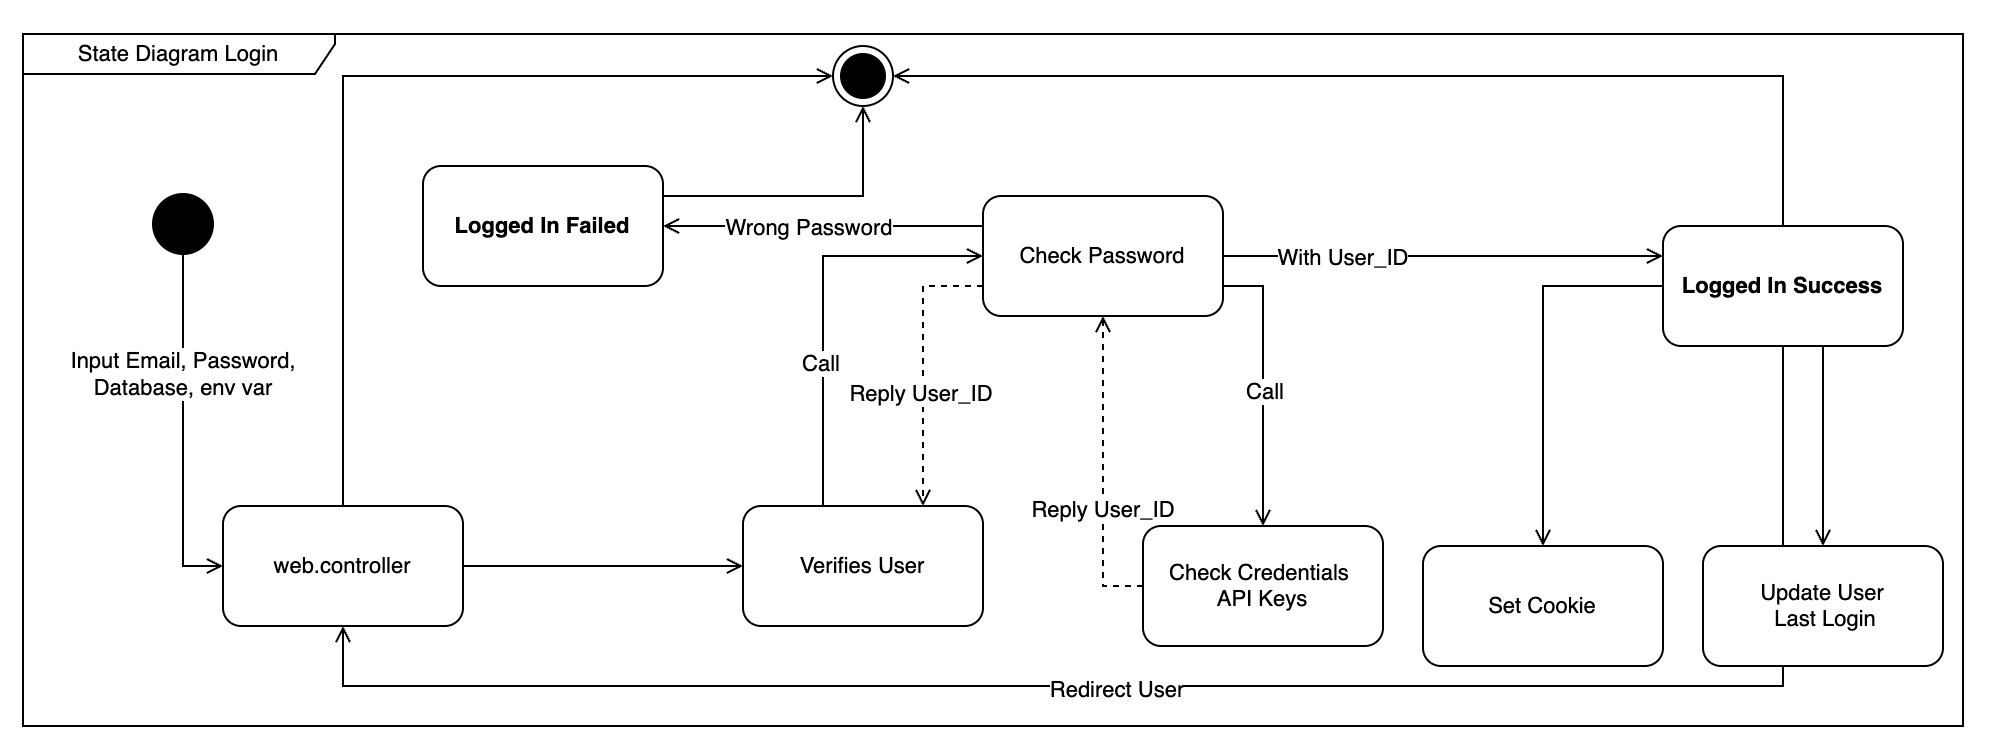
\includegraphics[width=14cm]{img/bab_3/stateDiagramLogin.png}
	\captionof{figure}{State Diagram pada proses login}
	\label{fig:asd}
\end{center}

Pada kasus bisnis untuk mendapatkan product, Odoo memiliki model framework yang memiliki fitur Object Relational Mapping(ORM), fitur controller dan fitur lainnya. Model framework diterapkan pada module addons ataupun odoo.addons, penggunaan model framework masih menjadi satu pada repo sehingga perubahan model dapat menyebabkan kerusakan di bagian addons lainnya. Model framework ini bisa diubah menjadi \textit{shared library} dan menjadi bentuk \textit{microservice chasis}.\\
\begin{center}
	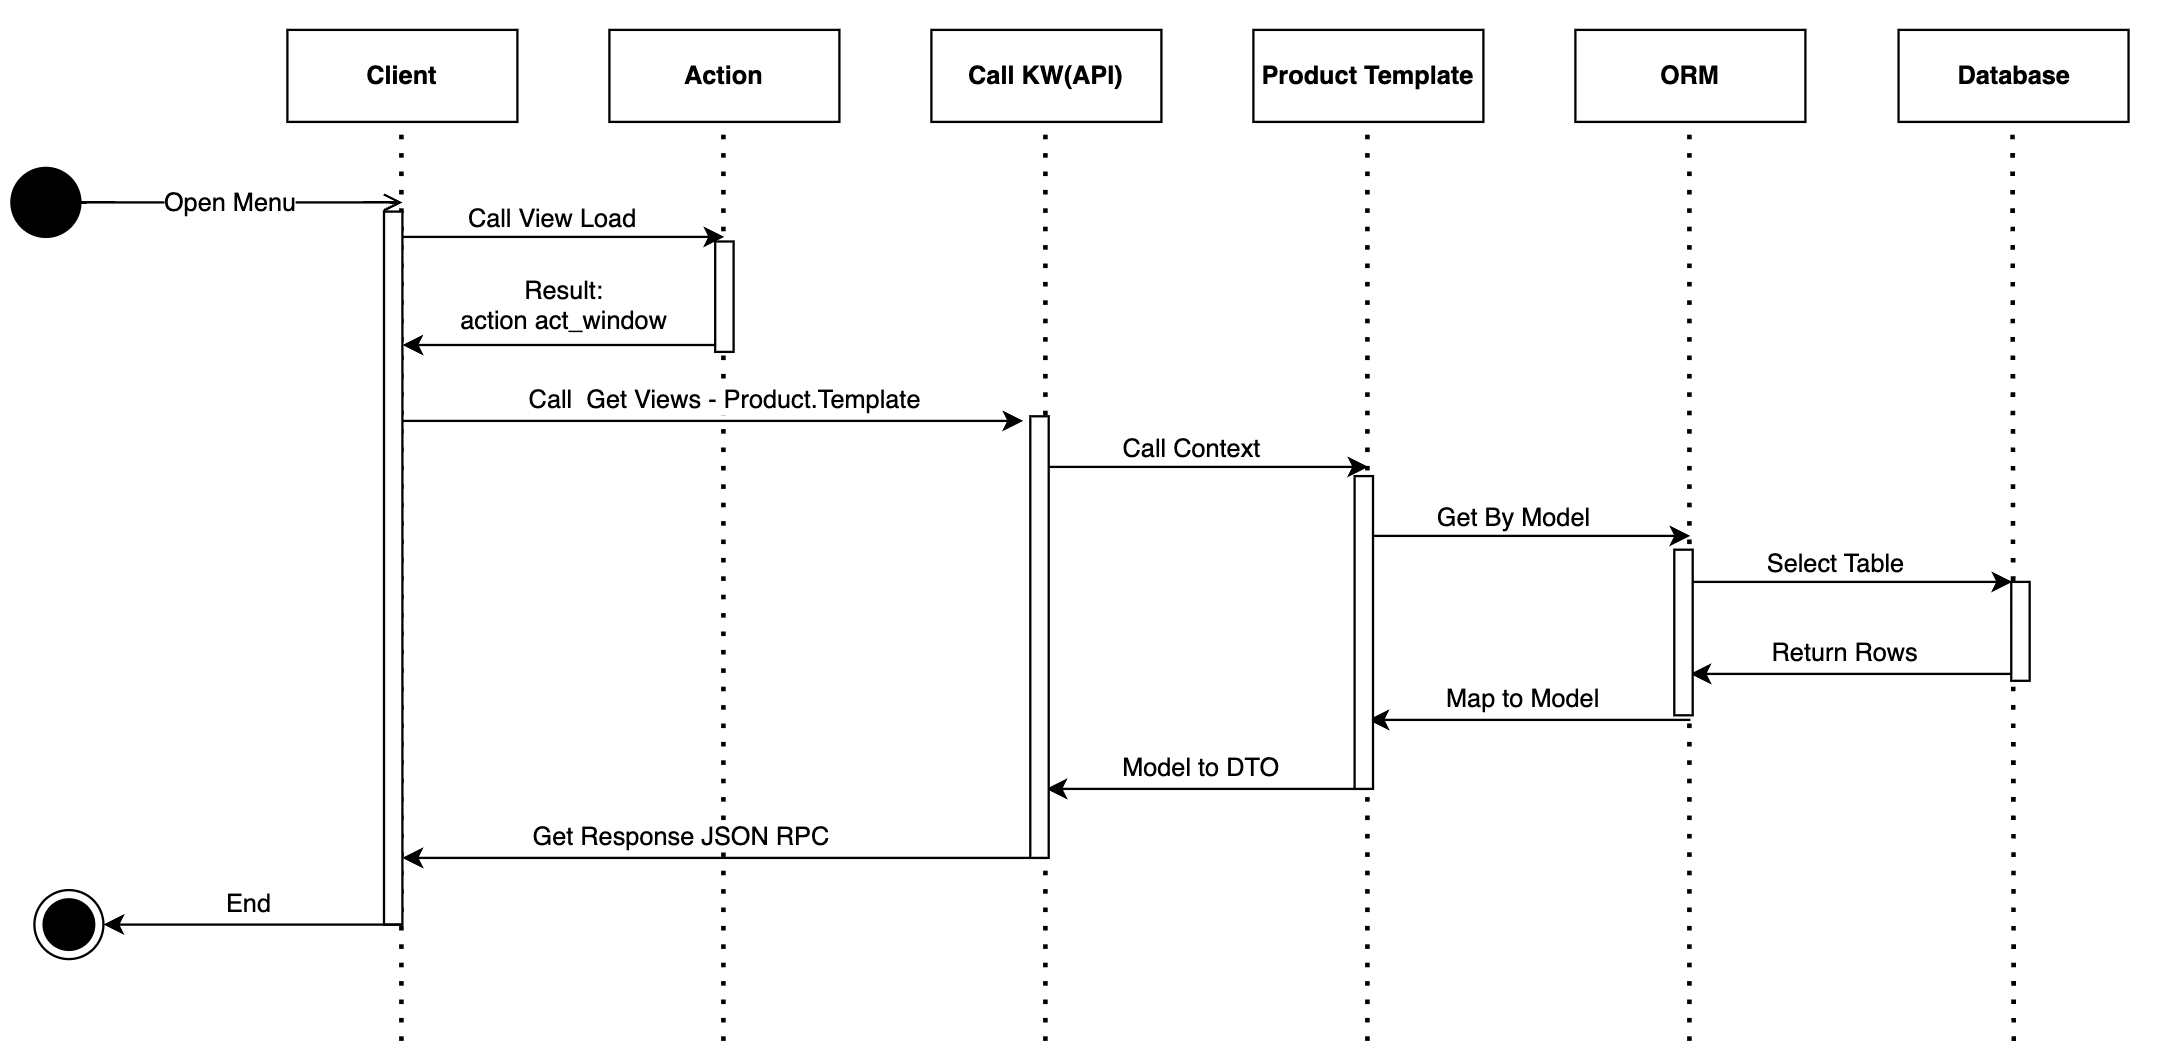
\includegraphics[width=14cm]{img/bab_3/seqDiagGet.png}
	\captionof{figure}{Sequence Diagram pada kasus pengambilan data Product}
	\label{fig:asd}
\end{center}
\subsubsection{Komunikasi antar service}
Proses komunikasi antar service dilakukan melalui JSON-RPC karena RPC ini sudah kompatibel dengan aplikasi monolit yang dibangun. Apabila diperlukan penambahan metode komunikasi lainnya seperti gRPC maka harus dibangun service yang mengubah gRPC menjad JSON-RPC atau sebaliknya.  
\\
\subsubsection{Strategi Pemisahan database}
Pemisahan database dilakukan bersama-sama dengan pemisahan kode karena pada Odoo sudah terdapat ORM yang mengelola database. Untuk menjaga konsistensi database antara service maka diterapkan SAGA dengan pendekatan Choreography. Untuk pengakses database monolit akan digunakan sebagai data access layer melalui API yang bisa berupa JSON-RPC. Proses seperti Insert, Update, Delete atau proses yang mengubah data maka harus melalui message broker agar pesan tidak hilang bila terjadi kegagalan disalah satu pihak. Untuk pengakses data seperti mencari dan mengambil data dapat melalui RPC.
\\
\subsection{Deployment}
\begin{center}
	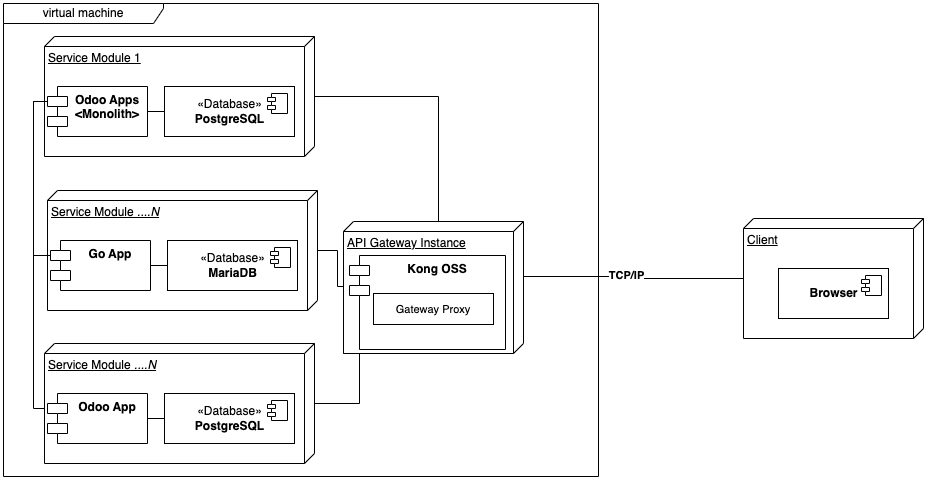
\includegraphics[width=14cm]{img/bab_3/Deployment.png}
	\captionof{figure}{Diagram Deployment}
	\label{fig:asd}
\end{center}
Tugas Akhir ini menggunakan API Gateway Kong \textit{(off-the-shelf)} karena Kong sudah memiliki fitur yang lengkap pada kasus migrasi aplikasi monolit ke microservice. Fitur itu berupa kemampuan untuk redireksi url untuk menerapkan proses strangle, adanya integrasi dengan Kubernetes untuk meningkatkan skalabilitas dan penemuan service, dan memiliki perfoma yang baik.